\documentclass{standalone}
\usepackage{tikz}
\usetikzlibrary{patterns, positioning}


\begin{document}
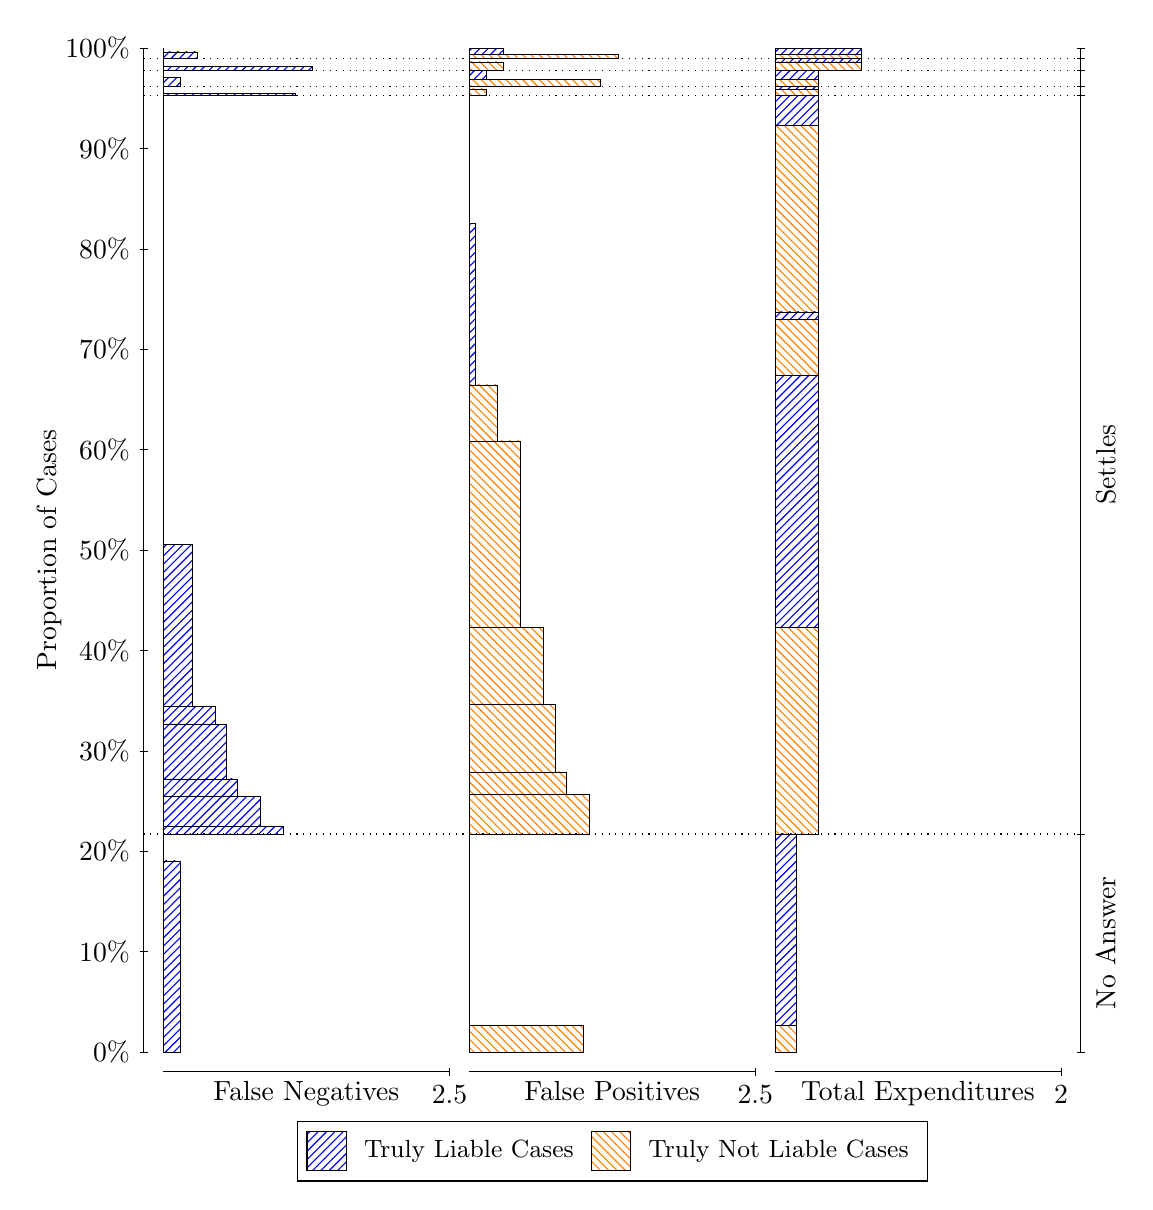
\begin{tikzpicture}
\draw[black, very thin] (1.5,1.75) -- (1.5,14.5);
\node[rotate=90, text=black, anchor=center] at (0.3, 8.125) {Proportion of Cases};
\draw[black, very thin] (1.45,1.75) -- (1.55,1.75);
\node[text=black, anchor=east] at (1.45, 1.75) {0\%};
\draw[black, very thin] (1.45,3.025) -- (1.55,3.025);
\node[text=black, anchor=east] at (1.45, 3.025) {10\%};
\draw[black, very thin] (1.45,4.3) -- (1.55,4.3);
\node[text=black, anchor=east] at (1.45, 4.3) {20\%};
\draw[black, very thin] (1.45,5.575) -- (1.55,5.575);
\node[text=black, anchor=east] at (1.45, 5.575) {30\%};
\draw[black, very thin] (1.45,6.85) -- (1.55,6.85);
\node[text=black, anchor=east] at (1.45, 6.85) {40\%};
\draw[black, very thin] (1.45,8.125) -- (1.55,8.125);
\node[text=black, anchor=east] at (1.45, 8.125) {50\%};
\draw[black, very thin] (1.45,9.4) -- (1.55,9.4);
\node[text=black, anchor=east] at (1.45, 9.4) {60\%};
\draw[black, very thin] (1.45,10.675) -- (1.55,10.675);
\node[text=black, anchor=east] at (1.45, 10.675) {70\%};
\draw[black, very thin] (1.45,11.95) -- (1.55,11.95);
\node[text=black, anchor=east] at (1.45, 11.95) {80\%};
\draw[black, very thin] (1.45,13.225) -- (1.55,13.225);
\node[text=black, anchor=east] at (1.45, 13.225) {90\%};
\draw[black, very thin] (1.45,14.5) -- (1.55,14.5);
\node[text=black, anchor=east] at (1.45, 14.5) {100\%};

\draw[black, very thin] (13.4,1.75) -- (13.4,14.5);
\draw[black, very thin] (13.35,1.75) -- (13.45,1.75);
\node[anchor=west] at (13.35, 1.75) {};
\draw[black, very thin] (13.35,4.5184) -- (13.45,4.5184);
\node[anchor=west] at (13.35, 4.5184) {};
\draw[black, very thin] (13.35,13.899) -- (13.45,13.899);
\node[anchor=west] at (13.35, 13.899) {};
\draw[black, very thin] (13.35,14.01) -- (13.45,14.01);
\node[anchor=west] at (13.35, 14.01) {};
\draw[black, very thin] (13.35,14.219) -- (13.45,14.219);
\node[anchor=west] at (13.35, 14.219) {};
\draw[black, very thin] (13.35,14.371) -- (13.45,14.371);
\node[anchor=west] at (13.35, 14.371) {};
\draw[black, very thin] (13.35,14.5) -- (13.45,14.5);
\node[anchor=west] at (13.35, 14.5) {};

\draw[black, very thin, pattern color=blue, pattern=north east lines] (1.75,1.75) rectangle (1.968,4.1774);
\draw[black, very thin, pattern color=orange, pattern=north west lines] (1.75,4.1774) rectangle (1.75,4.5184);
\draw[black, very thin, pattern color=blue, pattern=north east lines] (1.75,4.5184) rectangle (3.276,4.6168);
\draw[black, very thin, pattern color=blue, pattern=north east lines] (1.75,4.6168) rectangle (2.9853,4.9949);
\draw[black, very thin, pattern color=blue, pattern=north east lines] (1.75,4.9949) rectangle (2.6947,5.2181);
\draw[black, very thin, pattern color=blue, pattern=north east lines] (1.75,5.2181) rectangle (2.5493,5.9081);
\draw[black, very thin, pattern color=blue, pattern=north east lines] (1.75,5.9081) rectangle (2.404,6.1412);
\draw[black, very thin, pattern color=blue, pattern=north east lines] (1.75,6.1412) rectangle (2.1133,8.1949);
\draw[black, very thin, pattern color=orange, pattern=north west lines] (1.75,8.1949) rectangle (1.75,13.899);
\draw[black, very thin, pattern color=blue, pattern=north east lines] (1.75,13.899) rectangle (3.4213,13.928);
\draw[black, very thin, pattern color=orange, pattern=north west lines] (1.75,13.928) rectangle (1.75,14.01);
\draw[black, very thin, pattern color=blue, pattern=north east lines] (1.75,14.01) rectangle (1.968,14.124);
\draw[black, very thin, pattern color=orange, pattern=north west lines] (1.75,14.124) rectangle (1.75,14.219);
\draw[black, very thin, pattern color=blue, pattern=north east lines] (1.75,14.219) rectangle (3.6393,14.268);
\draw[black, very thin, pattern color=orange, pattern=north west lines] (1.75,14.268) rectangle (1.75,14.371);
\draw[black, very thin, pattern color=blue, pattern=north east lines] (1.75,14.371) rectangle (2.186,14.452);
\draw[black, very thin, pattern color=orange, pattern=north west lines] (1.75,14.452) rectangle (1.75,14.5);
\draw[black, very thin, pattern color=orange, pattern=north west lines] (5.6333,1.75) rectangle (7.0867,2.091);
\draw[black, very thin, pattern color=blue, pattern=north east lines] (5.6333,2.091) rectangle (5.6333,4.5184);
\draw[black, very thin, pattern color=orange, pattern=north west lines] (5.6333,4.5184) rectangle (7.1593,5.0214);
\draw[black, very thin, pattern color=orange, pattern=north west lines] (5.6333,5.0214) rectangle (6.8687,5.3082);
\draw[black, very thin, pattern color=orange, pattern=north west lines] (5.6333,5.3082) rectangle (6.7233,6.1622);
\draw[black, very thin, pattern color=orange, pattern=north west lines] (5.6333,6.1622) rectangle (6.578,7.1399);
\draw[black, very thin, pattern color=orange, pattern=north west lines] (5.6333,7.1399) rectangle (6.2873,9.5113);
\draw[black, very thin, pattern color=orange, pattern=north west lines] (5.6333,9.5113) rectangle (5.9967,10.223);
\draw[black, very thin, pattern color=blue, pattern=north east lines] (5.6333,10.223) rectangle (5.706,12.276);
\draw[black, very thin, pattern color=blue, pattern=north east lines] (5.6333,12.276) rectangle (5.6333,13.899);
\draw[black, very thin, pattern color=orange, pattern=north west lines] (5.6333,13.899) rectangle (5.8513,13.981);
\draw[black, very thin, pattern color=blue, pattern=north east lines] (5.6333,13.981) rectangle (5.6333,14.01);
\draw[black, very thin, pattern color=orange, pattern=north west lines] (5.6333,14.01) rectangle (7.3047,14.106);
\draw[black, very thin, pattern color=blue, pattern=north east lines] (5.6333,14.106) rectangle (5.8513,14.219);
\draw[black, very thin, pattern color=orange, pattern=north west lines] (5.6333,14.219) rectangle (6.0693,14.323);
\draw[black, very thin, pattern color=blue, pattern=north east lines] (5.6333,14.323) rectangle (5.6333,14.371);
\draw[black, very thin, pattern color=orange, pattern=north west lines] (5.6333,14.371) rectangle (7.5227,14.42);
\draw[black, very thin, pattern color=blue, pattern=north east lines] (5.6333,14.42) rectangle (6.0693,14.5);
\draw[black, very thin, pattern color=orange, pattern=north west lines] (9.5167,1.75) rectangle (9.7892,2.091);
\draw[black, very thin, pattern color=blue, pattern=north east lines] (9.5167,2.091) rectangle (9.7892,4.5184);
\draw[black, very thin, pattern color=orange, pattern=north west lines] (9.5167,4.5184) rectangle (10.062,7.1399);
\draw[black, very thin, pattern color=blue, pattern=north east lines] (9.5167,7.1399) rectangle (10.062,10.34);
\draw[black, very thin, pattern color=orange, pattern=north west lines] (9.5167,10.34) rectangle (10.062,11.051);
\draw[black, very thin, pattern color=blue, pattern=north east lines] (9.5167,11.051) rectangle (10.062,11.15);
\draw[black, very thin, pattern color=orange, pattern=north west lines] (9.5167,11.15) rectangle (10.062,13.521);
\draw[black, very thin, pattern color=blue, pattern=north east lines] (9.5167,13.521) rectangle (10.062,13.899);
\draw[black, very thin, pattern color=orange, pattern=north west lines] (9.5167,13.899) rectangle (10.062,13.981);
\draw[black, very thin, pattern color=blue, pattern=north east lines] (9.5167,13.981) rectangle (10.062,14.01);
\draw[black, very thin, pattern color=orange, pattern=north west lines] (9.5167,14.01) rectangle (10.062,14.106);
\draw[black, very thin, pattern color=blue, pattern=north east lines] (9.5167,14.106) rectangle (10.062,14.219);
\draw[black, very thin, pattern color=orange, pattern=north west lines] (9.5167,14.219) rectangle (10.607,14.323);
\draw[black, very thin, pattern color=blue, pattern=north east lines] (9.5167,14.323) rectangle (10.607,14.371);
\draw[black, very thin, pattern color=orange, pattern=north west lines] (9.5167,14.371) rectangle (10.607,14.42);
\draw[black, very thin, pattern color=blue, pattern=north east lines] (9.5167,14.42) rectangle (10.607,14.5);
\draw[black, dotted] (1.5,4.5184) -- (13.4,4.5184);
\draw[black, dotted] (1.5,13.899) -- (13.4,13.899);
\draw[black, dotted] (1.5,14.01) -- (13.4,14.01);
\draw[black, dotted] (1.5,14.219) -- (13.4,14.219);
\draw[black, dotted] (1.5,14.371) -- (13.4,14.371);
\draw[black, very thin] (1.75,1.5) -- (5.3833,1.5);
\node[text=black, anchor=north] at (3.5667, 1.5) {False Negatives};
\draw[black, very thin] (5.3833,1.45) -- (5.3833,1.55);
\node[text=black, anchor=north] at (5.3833, 1.45) {2.5};

\draw[black, very thin] (5.6333,1.5) -- (9.2667,1.5);
\node[text=black, anchor=north] at (7.45, 1.5) {False Positives};
\draw[black, very thin] (9.2667,1.45) -- (9.2667,1.55);
\node[text=black, anchor=north] at (9.2667, 1.45) {2.5};

\draw[black, very thin] (9.5167,1.5) -- (13.15,1.5);
\node[text=black, anchor=north] at (11.333, 1.5) {Total Expenditures};
\draw[black, very thin] (13.15,1.45) -- (13.15,1.55);
\node[text=black, anchor=north] at (13.15, 1.45) {2};

\node[text=black, centered, rotate=90] at (13.72, 3.1342) {No Answer};
\node[text=black, centered, rotate=90] at (13.72, 9.2088) {Settles};





\draw (7.449999999999999,1.5) node[draw=none] (baseCoordinate) {};
\begin{scope}[align=center]
        \matrix[scale=0.5, draw=black, below=0.5cm of baseCoordinate, nodes={draw}, column sep=0.1cm]{
            \node[rectangle, draw, minimum width=0.5cm, minimum height=0.5cm, pattern color=blue, pattern=north east lines] {}; &
            \node[draw=none, font=\small, text=black] (B) {Truly Liable Cases}; &
            \node[rectangle, draw, minimum width=0.5cm, minimum height=0.5cm, pattern color=orange, pattern=north west lines] {}; &
            \node[draw=none, font=\small, text=black] (B) {Truly Not Liable Cases}; \\
            };
\end{scope}

\end{tikzpicture}
\end{document}